\documentclass[professionalfonts, xcolor={usenames,svgnames,x11names,table}]{beamer}

\usetheme{SBUclass}
\usepackage{mypackages}
\usepackage{mycommands}


\title{\texorpdfstring{Language \& Technology}{Language and Technology}}
\subtitle{Lecture 4: More Word-Based Models}
\author{Al{\"e}na Aks{\"e}nova \& Aniello De Santo}
\institute{Stony Brook University\\\texttt{alena.aksenova@stonybrook.edu}\\\texttt{aniello.desanto@stonybrook.edu}}
\date{}



\begin{document}
\unnumbered{
\begin{frame}
	\titlepage
\end{frame}
}
%
\begin{frame}{Previously on ``Language \& Technology''\ldots}
    \begin{itemize}
        \item Counting words!
    \end{itemize}
 \begin{description}
    \item[string] = "The sun shone, having no alternative, on the nothing new."
   \item[tokens] ["the", "sun", "shone", "having", "no", "alternative", "on", "the", "nothing", "new"]
\end{description}

    \begin{itemize}
        \item More technically: for each word type we count its word tokens.
    \end{itemize}
    \begin{description}
        \item[word type] a word of a given language
        \item[word token] instance of the word in a text
    \end{description}
\end{frame}

\begin{frame}{Previously on ``Language \& Technology''\ldots}
    \begin{block}{Steps of Word Counting Model}
        \begin{enumerate}
            \item collect corpus
            \item tokenize strings
            \item count tokens for each type
        \end{enumerate}
    \end{block}

    \pause
    Counting words is surprisingly useful:
    %
    \begin{itemize}
        \item Culturomics
        \item Stylistic analysis
    \end{itemize}
    %
    But there's more!
\end{frame}

\begin{frame}{Application 3: Authorship Attribution}
    \begin{itemize}
        \item Computational stylistic analysis isn't just good at\\
            predicting success of novels.
        \item Word counts pick up on \highlight{statistical tendencies in writing} of individual authors
        \item This means that potential authors can be inferred from\\
             word frequencies!
    \end{itemize}
\end{frame}

\begin{frame}{Example: Auditing the Bard's Oeuvre}
    \begin{columns}
        \column{.7\linewidth}
        \begin{itemize}
            \item Several works of Shakespeare have supposedly been (partially) authored by somebody else:
                \begin{itemize}
                    \item \emph{Edward III}\\
                        co-authored with Thomas Kyd
                    \item \emph{The Comedy of Errors},\\
                        \emph{Love's Labour Lost},\\
                        \emph{The Tempest}\\
                        co-authored with Francis Bacon
                \end{itemize}
            \item These are \highlight{fringe ideas} in literary circles.
            \item But there are word counting models that \highlight{support these claims}.
        \end{itemize}

        \column{.3\linewidth}
        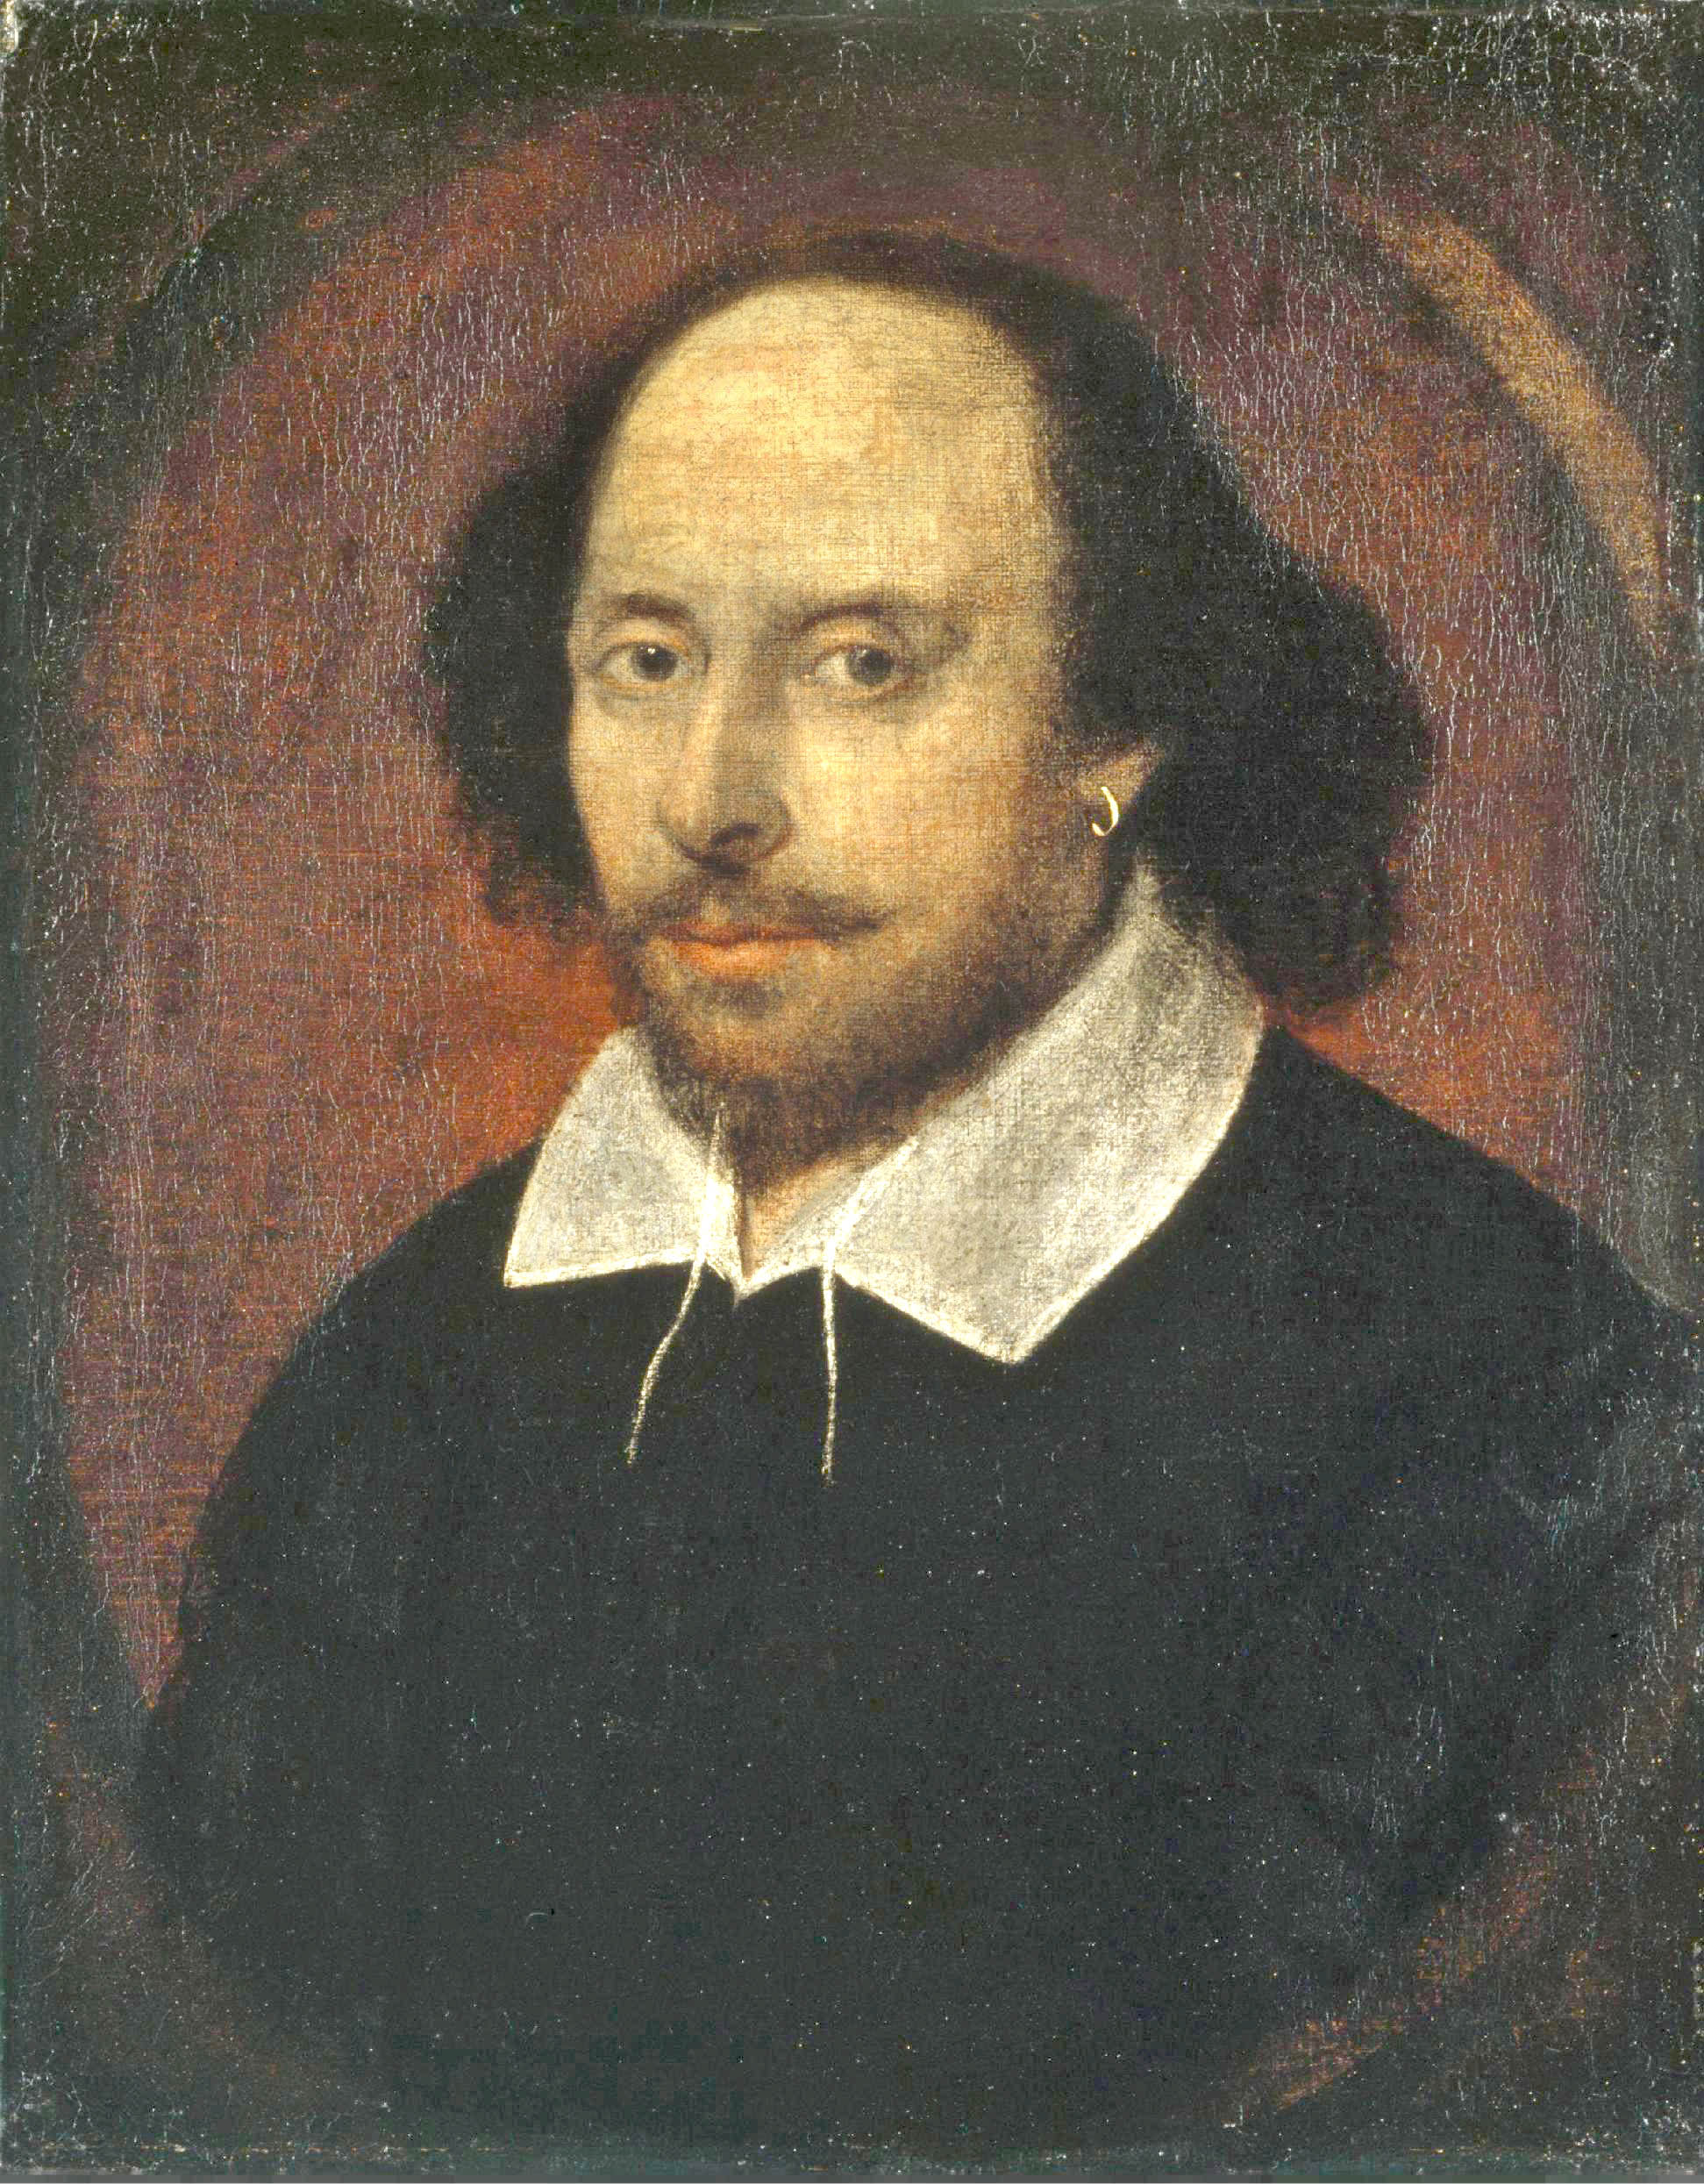
\includegraphics[width=1\linewidth]{./img/shakespeare}
    \end{columns}
\end{frame}

\begin{frame}{Another Example: Harry Potter's Mum}
    \begin{columns}
        \column{.6\linewidth}
        \begin{itemize}
            \item New book: \emph{The Cuckoo's Calling} by Robert Galbraith
            \item \emph{Sunday Times} suspected that to be a pseudonym for J.~K.~Rowling.
            \item Evidence from word-based model: 
            \begin{itemize}
                \item 100 most common words
                \item average word length
                \item word pairs\\
                    \subpoint{(discussed in next lecture)}
                \item character 4-grams\\
                    \subpoint{(discussed in next lecture)}
            \end{itemize}
        \end{itemize}

        \column{.33\linewidth}
        \centering
        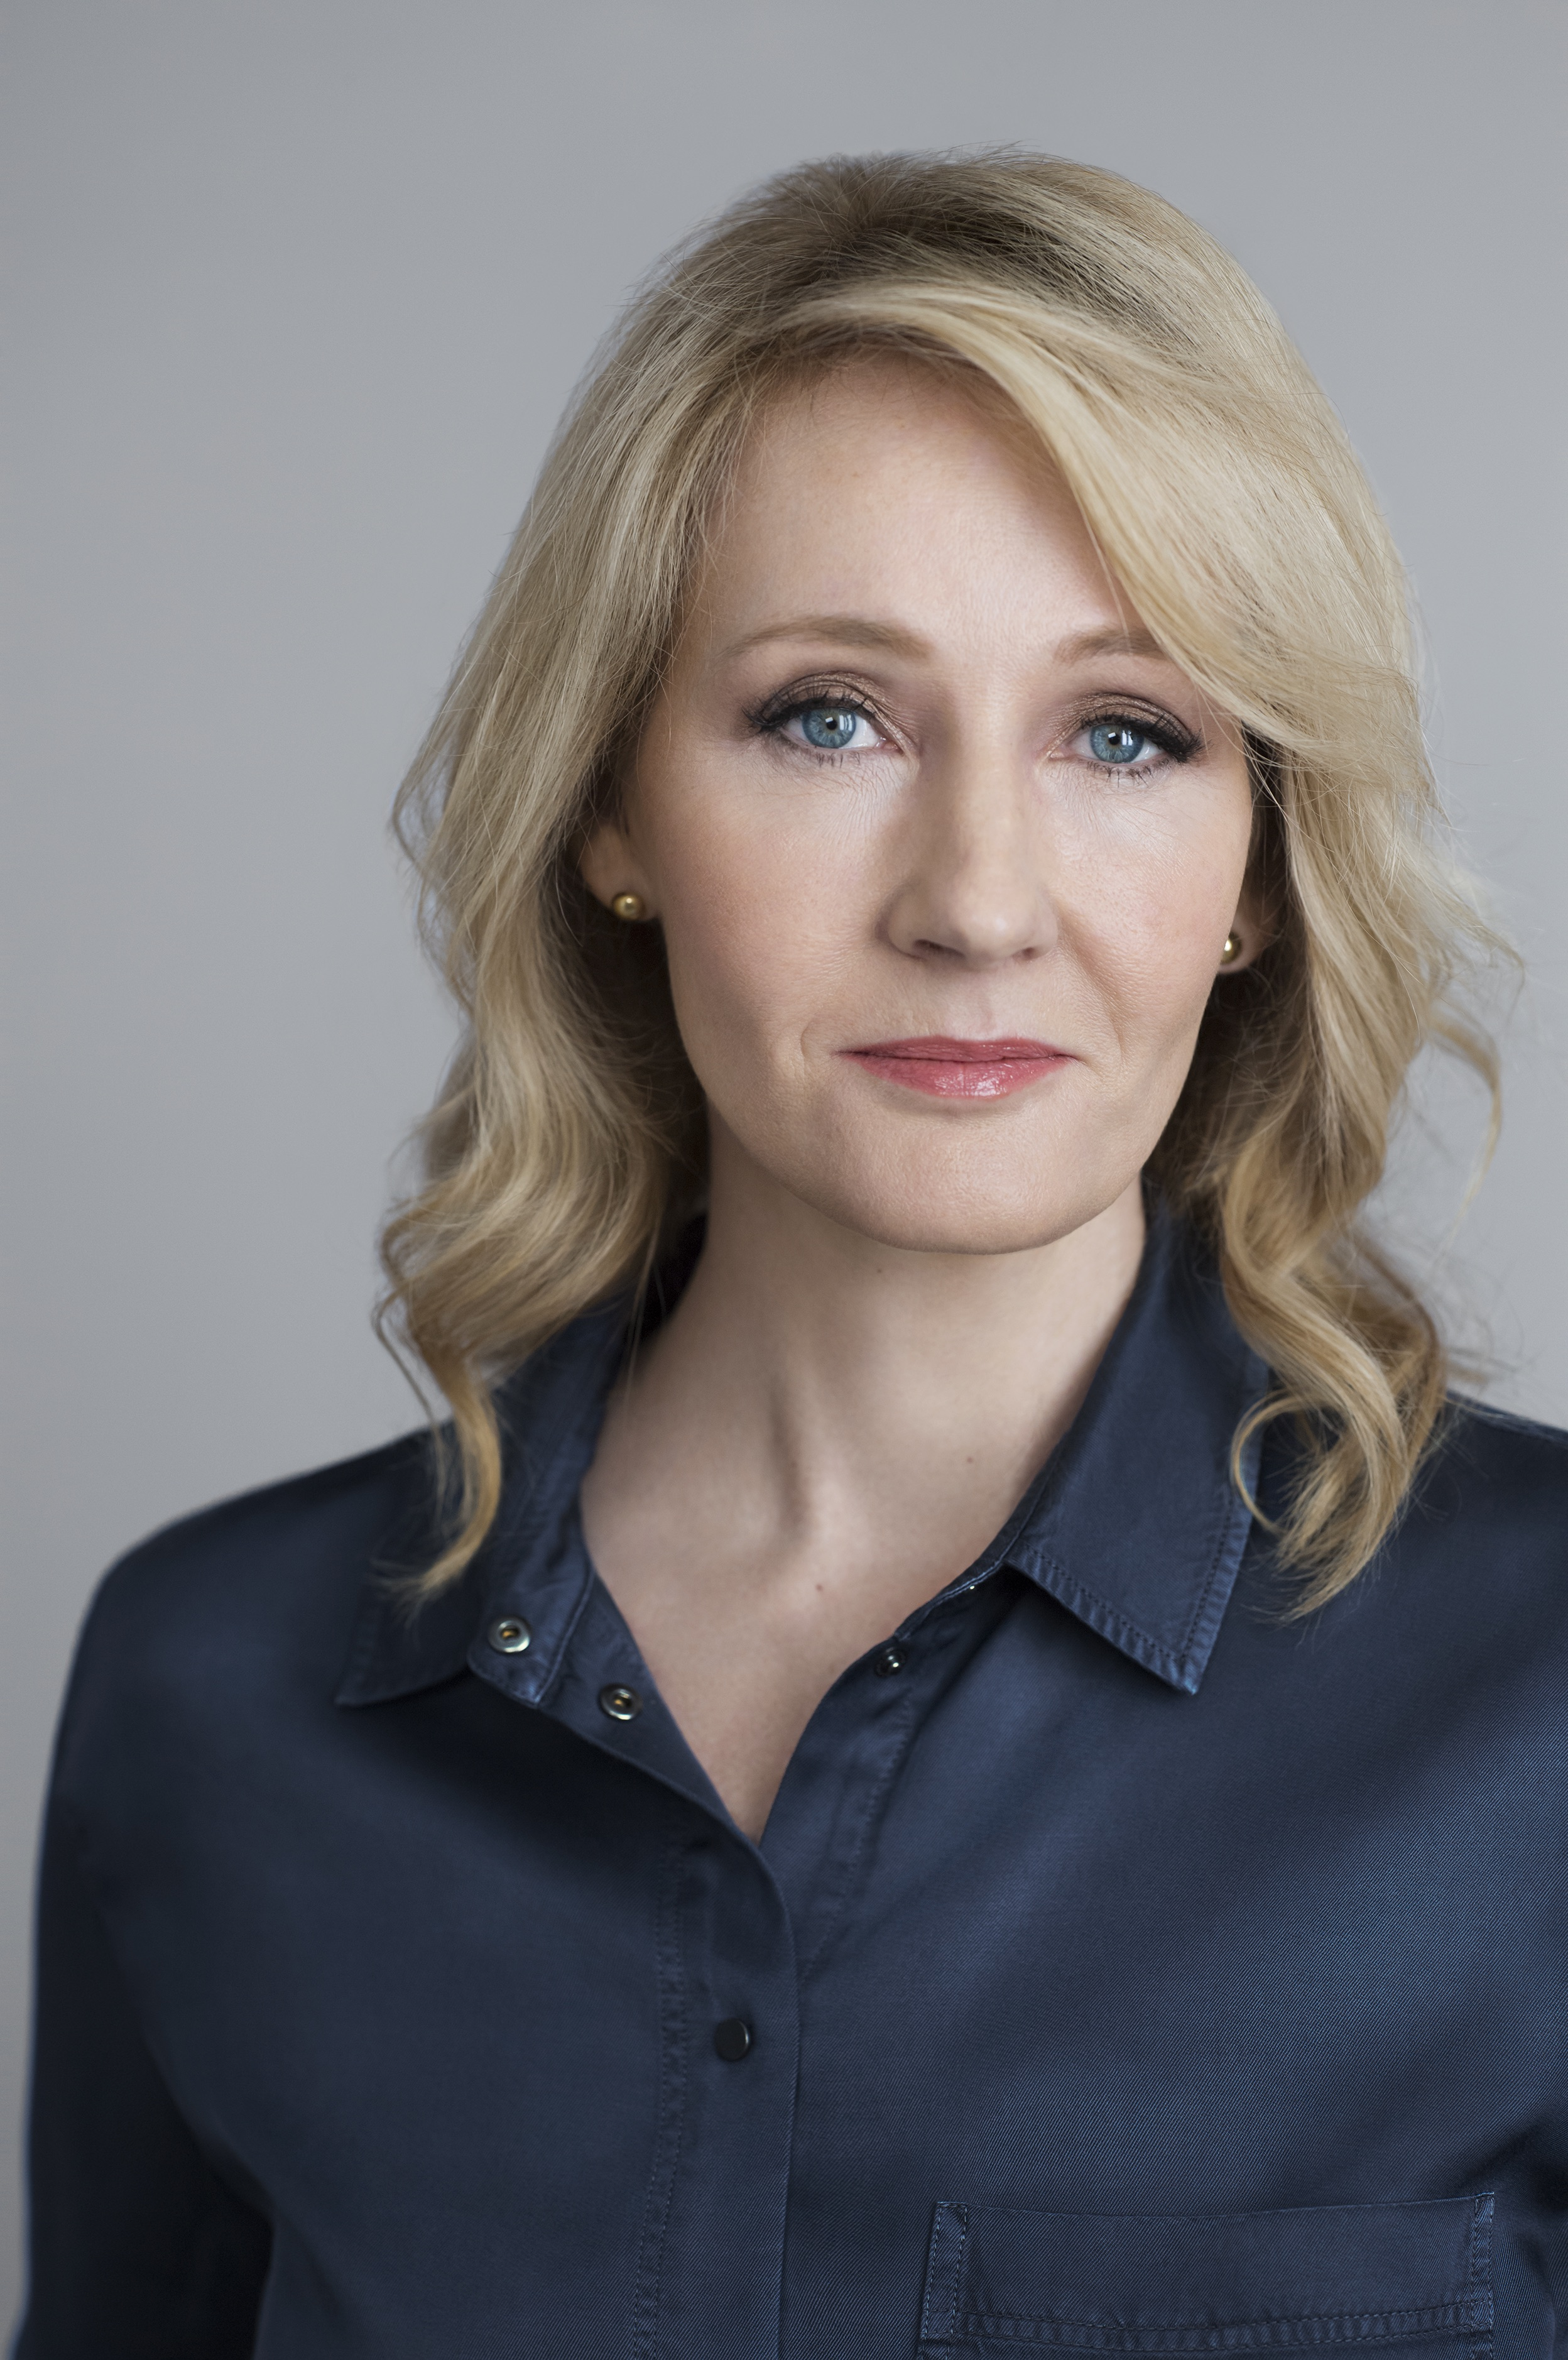
\includegraphics[width=1\linewidth]{./img/jkrowling}
    \end{columns}
    \begin{followup}
        Article on \href{http://languagelog.ldc.upenn.edu}{LanguageLog}: \url{http://languagelog.ldc.upenn.edu/nll/?p=5315}
    \end{followup}
\end{frame}

\begin{frame}{Evaluation}
    \begin{itemize}
        \item As with culturomics, it is unclear what to make of\\
            the findings.
            \begin{itemize}
                \item J.K. Rowling: success!
                \item Shakespeare: success?
            \end{itemize}
        \item One can get vastly different results depending on:
            \begin{itemize}
                \item absolute size of test corpus
                \item relative size (e.g.\ ratio of Shakespeare to Bacon)
                \item whether certain words are ignored
                \item whether one pays attention to rare words or frequent words
            \end{itemize}
        \item Many of these studies feel backwards:
            \begin{itemize}
                \item They start with a specific hypothesis and then present\\
                    one specific model that supports this hypothesis.
                \item But why is this model better than all of the alternatives?
            \end{itemize}
    \end{itemize}
\end{frame}

\begin{frame}{Moral of the Story}
    \begin{itemize}
        \item Authorship attribution models still ill-understood
        \item In the future, these models might answer long-standing questions or pose new ones.
        \item Maybe you can try it in an English class.
    \end{itemize}
\end{frame}


\begin{frame}{Application 4: Word Meanings}
    \begin{itemize}
        \item For some tasks, the word types are not that important,\\
            what matters is their \highlight{meaning}:
            \begin{itemize}
                \item web search
                \item Google \emph{Ad Sense} (automatic ad placement)
            \end{itemize}
        \item But what is a word meaning?
    \end{itemize}

\visible<2->{
    \begin{exampleblock}{Example: Dictionary Approach}
        \textbf{dog}
        \begin{itemize}
            \item is a \textbf{mammal},
            \item descended from \textbf{wolf},
            \item is commonly a \textbf{pet},
            \item subtypes are \textbf{poodle}, \textbf{bulldog}, \ldots
            \item has \textbf{fur},
            \item \ldots
        \end{itemize}
    \end{exampleblock}
    }
    % fixme: use wordnet here
\end{frame}

\begin{frame}{Why the Dictionary Approach is Problematic}
    \begin{itemize}
        \item Such dictionaries have been tried for computers.\\
            \subpoint{e.g. \href{https://wordnet.princeton.edu/}{WordNet}}
        \item They must be created by hand, which is a big problem:
            \begin{itemize}
                \item expensive
                \item only available for some languages
                \item many new words missing
            \end{itemize}
        \item We need dictionaries that can be generated automatically.
    \end{itemize}
\end{frame}

\begin{frame}{Meaning as Word Use}
    \begin{columns}
        \column{.7\linewidth}
        \begin{itemize}
            \item The philosopher \textbf{Ludwig Wittgenstein} said that a word's meaning is its use.
        \end{itemize}
        \begin{block}{Computational Counterpart}
            A word's meaning is given by how often it occurs together with other words.
        \end{block}
        
        \column{.3\linewidth}
        \centering
        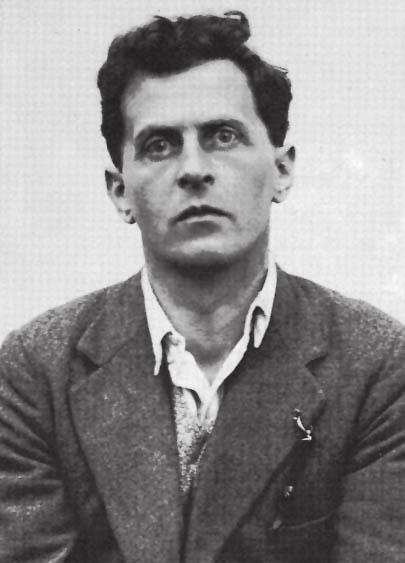
\includegraphics[width=1\linewidth]{./img/wittgenstein}
    \end{columns}
\end{frame}

\begin{frame}{Counting Tokens for Word Meaning}
    \textbf{Step 1:} Record in how many sentences words \highlight{occur together}
    %
    \begin{example}
        \begin{quote}
            The dog barked at the cat.
            The cat ran away.
            The dog ran after the cat.
            The dog kept barking.
            He also kept running.
        \end{quote}
        %
        \centering
            \begin{tabular}{r|cccc}
                           & dog & cat & bark & run\\
                    \hline
                    dog    & -   & \visible<2->{2}   & \visible<3->{2}    & \visible<4->{1}\\
                    cat    & \visible<5->{2}   & -   & \visible<6->{1}    & \visible<7->{2}\\
                    bark   & \visible<8->{2}   & \visible<9->{1}   & -    & \visible<10->{0}\\ 
                    run    & \visible<11->{1}   & \visible<12->{2}   & \visible<13->{0}    & -\\
            \end{tabular}
    \end{example}
\end{frame}

\begin{frame}{From Vector to Vector Spaces}
    \textbf{Step 2:} Construct an $n$-dimensional vector space.\\
    \subpoint{\qquad\qquad $n$ is given by the number of word types in the text}
    %
    \begin{exampleblock}{2-Dimensional Vector Space with \emph{dog} and \emph{cat}}
        %
        \begin{columns}
            \column{.3\linewidth}
            \centering
                \begin{tikzpicture}
                    \node (top) at (0em,10em) {};
                    \node (start) at (0,0) {};
                    \node (right) at (10em,0em) {};

                    \foreach \x in {4em,8em}
                        {
                        \draw[gray] (\x, .25em) -- (\x, -.25em);
                        \draw[gray] (.25em, \x) -- (-.25em, \x);
                        }

                    \draw[->,gray] (start.center) to node [above,pos=1] {dog} (top);
                    \draw[->,gray] (start.center) to node [right,pos=1] {cat} (right);

                    \draw[->,SteelBlue4] (start.center) to node [left, pos=.9] {bark} (4em,8em);
                    \draw[->,Red3] (start.center) to node [below, pos=.9] {run} (8em,4em);
                \end{tikzpicture}

            \column{.55\linewidth}
            \begin{center}
                \begin{tabular}{r|cccc}
                               & dog & cat & bark & run\\
                        \hline
                        dog    & -   & {2}   & {2}    & {1}\\
                        cat    & {2}   & -   & {1}    & {2}\\
                        bark   & \tikz[overlay,remember picture, baseline=-.7ex]{\node (bd) {2};}
                               & \tikz[overlay,remember picture, baseline=-.7ex]{\node (bc) {1};}
                               & -    & {0}\\ 
                        run    & \tikz[overlay,remember picture, baseline=-.7ex]{\node (rd) {1};}
                               & \tikz[overlay,remember picture, baseline=-.7ex]{\node (rc) {2};}
                               & {0}    & -\\
                \end{tabular}
                \begin{tikzpicture}[overlay, remember picture]
                    \draw[draw=Purple, fill=Purple, thick, fill opacity=.25]
                        (bd.north west) rectangle (rc.south east);
                \end{tikzpicture}
            \end{center}
            \begin{itemize}
                \item \emph{bark} more closely related to \emph{dog}
                \item \emph{run} more closely related to \emph{cat}
            \end{itemize}
        \end{columns}
    \end{exampleblock}
\end{frame}

\begin{frame}{From Word Meaning to Text Meaning}
    \textbf{Step 3}: construct vector for whole text from word vectors

    \begin{exampleblock}{Meaning for \emph{He either barks or runs and barks}}
        \centering
        \begin{tikzpicture}
            \node (top) at (0em,10em) {};
            \node (start) at (0,0) {};
            \node (right) at (10em,0em) {};

            \foreach \x in {4em,8em}
                {
                \draw[gray] (\x, .25em) -- (\x, -.25em);
                \draw[gray] (.25em, \x) -- (-.25em, \x);
                }

            \draw[->,gray] (start.center) to node [above,pos=1] {dog} (top);
            \draw[->,gray] (start.center) to node [right,pos=1] {cat} (right);

            \draw[->,SteelBlue4] (start.center) to node [left, pos=.9] {bark} (4em,8em);
            \draw[->,Red3] (start.center) to node [below, pos=.9] {run} (8em,4em);
            \draw[->,Purple] (start.center) to node [right, pos=.9] {text} (5em,7em);
        \end{tikzpicture}
    \end{exampleblock}
\end{frame}

\begin{frame}{Is that Realistic?}
    \begin{itemize}
        \item \textbf{Possible Concerns}
            \begin{itemize}
                \item Is word meaning really just a bunch of numbers?
                \item In a real-word model, the vector space will have\\
                    thousands of dimensions.
            \end{itemize}
        \item But this might actually be what you have stored in your brain!
    \end{itemize}
    %
    \begin{block}{Psycholinguistic Experiment}
        \begin{itemize}
            \item Word association task
            \item The more similar the meaning vectors of two words,\\
                the faster test subjects recognize them as related.
               \item Also: \href{http://www.u.arizona.edu/~kforster/priming/index.htm}{Masked priming effects}
        \end{itemize}
    \end{block}
\end{frame}

\begin{frame}{Usage for Web Search and Ad Sense}
    \begin{itemize}
        \item \textbf{Web Search}
            \begin{itemize}
                \item construct meaning vector for every website
                \item convert search string to vector
                \item rank websites by vector similarity
            \end{itemize}
        \item \textbf{Ad Sense}
            \begin{itemize}
                \item construct meaning vector for every website
                \item associate every ad with a vector
                \item pick ad that most closely matches website vector
            \end{itemize}
    \end{itemize}

    \begin{block}{Bells and Whistles}
        \begin{itemize}
            \item weigh words in search string by linear order\\
                \subpoint{aliens conspiracy $\neq$ conspiracy aliens}
            \item prioritize certain words in text
            \item compress vector space for efficiency
        \end{itemize}
    \end{block}
\end{frame}

\begin{frame}{Evaluation}
    \begin{itemize}
        \item For word meaning, the approach seems to work.
        \item But it is bad for sentence/text meaning.
    \end{itemize}
    %
    \begin{example}
        The following two sentences receive the same vector:
        %
        \begin{exe}
            \ex
            \begin{xlist}
                \ex Dog bites man!
                \ex Man bites dog!
            \end{xlist}
        \end{exe}
    \end{example}
    %
    \begin{followup}
        How meaning actually works: \textbf{LIN 346 Language and Meaning}
    \end{followup}
\end{frame}

\begin{frame}{An Observation on Frequencies: Zipf's Law}
    \begin{columns}
        \column{.5\linewidth}    
        \begin{itemize}
            \item Word models care about word frequency.
            \item But there is a problem\ldots
        \end{itemize}
        %
        \begin{alertblock}{Zipf's Law}
            The frequency of a type is inversely proportional to its rank.
        \end{alertblock}

        \column{.38\linewidth}    
        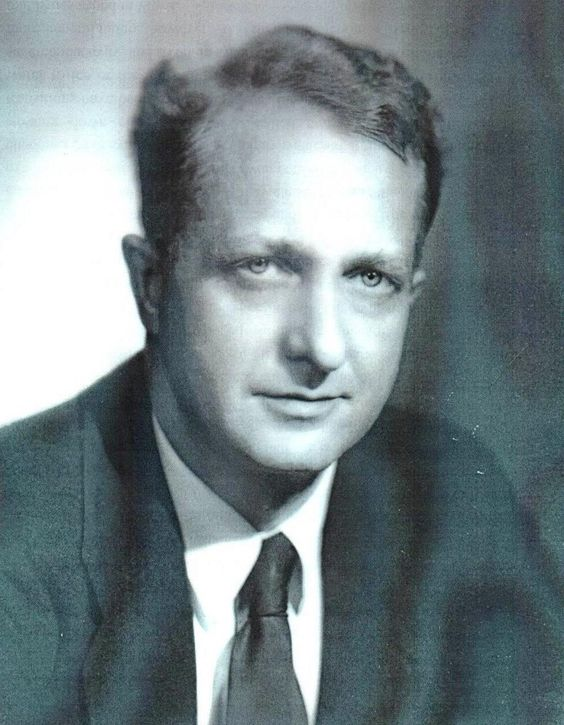
\includegraphics[width=.8\linewidth]{./img/george_zipf}
    \end{columns}

    \pause
    \begin{block}{In Plain English}
        The most frequent word is
            \begin{itemize}
                \item \colored{blue!75}{\textbf{2}} times as common as the \colored{blue!75}{\textbf{2}}nd most frequent word,
                \item \colored{orange}{\textbf{3}} times as common as the \colored{orange}{\textbf{3}}rd most frequent word,
                \item and so on.
            \end{itemize}
    \end{block}
\end{frame}

\begin{frame}{An Example from\ldots the NBA?}
    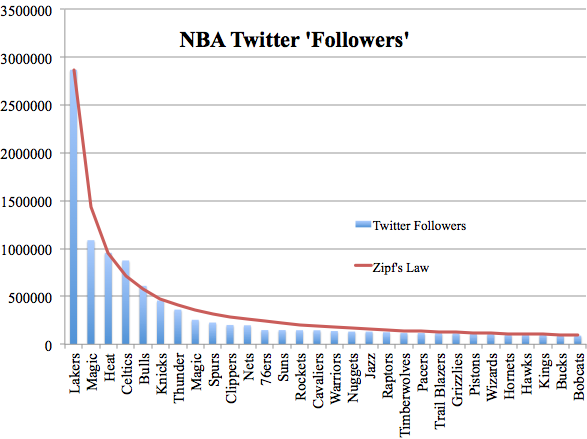
\includegraphics[width=.9\linewidth]{./img/zipfgraph_nba}
\end{frame}


\begin{frame}{Visualizing Zipf Distributions}
    \centering
    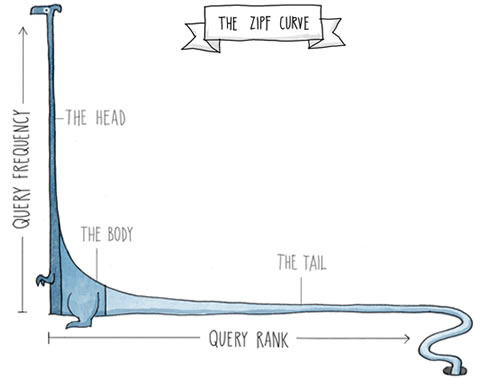
\includegraphics[width=.8\linewidth]{./img/zipfgraph_dinosaur}
\end{frame}

\begin{frame}{Zipf's Law is Everywhere\ldots}
    \begin{itemize}
        \item A distribution is probably Zipfian if
            \begin{itemize}
                \item there is a \highlight{long neck}:\\
                    a few types make up the majority of tokens,
                \item there is a \highlight{long tail}:\\
                    most types only have 1 token (\textbf{hapax legomenon})
            \end{itemize}
        \item Surprisingly, Zipf's Law shows up in tons of places:
            \begin{itemize}
                \item size of large cities in a country
                \item citations for academic papers
                \item frequencies of last names
                \item frequencies of weekdays in text
            \end{itemize}
    \end{itemize}
\end{frame}

\begin{frame}{\ldots Even in Language!}
    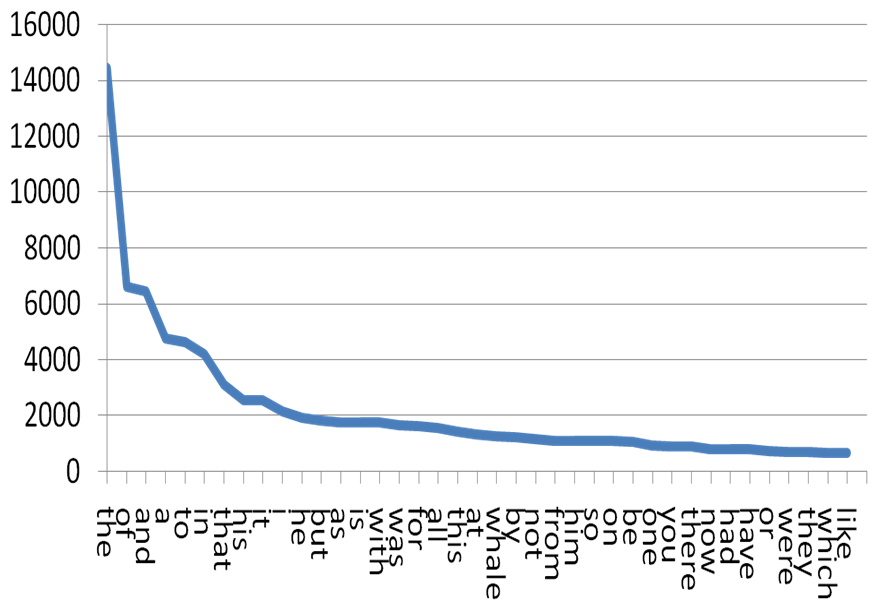
\includegraphics[width=.9\linewidth]{./img/zipfgraph_english}
\end{frame}

\begin{frame}{Stop Words}
    \begin{itemize}
        \item About 150 words make up 50\% of all English texts:\\
            \emph{the}, \emph{of}, \emph{and}, \emph{a}, \ldots
        \item These are called \highlight{stop words}.
        \item Stop words are not very informative for many applications.
        \item So they are usually discarded after the tokenization step.
        \item Failure to do so can greatly reduce the model's performance. 
    \end{itemize}

    \pause
    \begin{block}{Steps of Word Counting Model (Revised)}
        \begin{enumerate}
            \item collect corpus
            \item remove stop words
            \item tokenize strings
            \item count tokens for each type
        \end{enumerate}
    \end{block}
\end{frame}

\begin{frame}{Example: A Text Without (Non)-Stop Words}
    \begin{itemize}
        \item Stop words are much less informative than non-stop words.
        \item Just check the example below.
    \end{itemize}

    \only<1>{\textbf{Stop Words only}}%
    \only<2>{\textbf{Stop Words and Non-Stop Words}}%
    \only<3>{\textbf{Non-Stop Words only}}%

    \bigskip
    \visible<1,2>{The}
    \visible<2,3>{sun}
    \visible<2,3>{shone}
    \visible<1,2>{having}
    \visible<1,2>{no}
    \visible<2,3>{alternative}
    \visible<1,2>{on}
    \visible<1,2>{the}
    \visible<2,3>{nothing}
    \visible<2,3>{new}
\end{frame}

\begin{frame}{An Important Consequence of Zipf's Law}
    \begin{itemize}
        \item Texts mostly consist of stop words.
        \item Hence it can be difficult to get representative counts\\
            for non-stop words.
    \end{itemize}
    %
    \begin{block}{Sparse Data Problem}
        \begin{itemize}
            \item Most of the data is not informative.
            \item You need tons of data to have enough useful data.
        \end{itemize}
    \end{block}
    %
    \visible<2>{
    \begin{example}
        \begin{itemize}
            \item Most models require corpora with at least\\
                a few million sentences.
            \item Really good models (e.g. Google translate) use\\
                billions of data points.
        \end{itemize}
    \end{example}
    }
\end{frame}

\begin{frame}{Summary}
    \begin{itemize}
        \item Unigram (= word-based) models are surprisingly useful.
            \begin{itemize}
                \item culturomics
                \item stylistic analysis
                \item authorship attribution
                \item word meaning
                \item web search
                \item ad sense
                \item and much more
            \end{itemize}
        \item They just count words and do some number crunching with the frequencies.
        \item These models are everywhere, but they are also very simplistic.
        \item Quality depends largely on how much data is available.
    \end{itemize}
\end{frame}

\end{document}

n-gram models
    word prediction
    where it would help: ocr
